\documentclass[12pt]{article}
\usepackage[a4paper,
            inner=10mm,
            outer=50mm, % = marginparsep + marginparwidth 
                       %   + 5mm (between marginpar and page border)
            top=20mm,
            bottom=25mm,
            marginparsep=5mm,
            marginparwidth=40mm,
            % showframe
            ]{geometry}
\usepackage{amsfonts}
\usepackage{amsmath}
\usepackage{xcolor}
\usepackage{todonotes}
\usepackage{pythonhighlight}
\usepackage{fancyvrb}
\usepackage{minted}

% define command for grey colored text
% \newcommand{\note}[1]{ \textit{\textcolor{gray}{... #1 ...}} }
\newcommand{\note}[1]{\todo[color=yellow!40,bordercolor=none,linecolor=black]{~~ #1}}
\tolerance=1
\emergencystretch=\maxdimen
\hyphenpenalty=10000
\hbadness=10000

\newcommand{\includecode}[2]{
\begin{listing}[H]
    \caption{#2}
    \label{code:#1}
    \inputminted[frame=single, framesep=10pt, fontsize=\footnotesize]{python}{src/#1.py}
\end{listing}   
}
\renewcommand\listingscaption{Pseudo-code}


\newcommand{\argmax}[1]{\operatorname*{argmax}_{#1}}

\usepackage{tikz}
\newcommand*\circled[1]{\tikz[baseline=(char.base)]{
            \node[shape=circle,draw,inner sep=2pt] (char) {#1};}}

% bibilography management
\usepackage[style=numeric]{biblatex}
\addbibresource{main.bib}

\begin{document}

\listoftodos

\tableofcontents

\section{Summary of Notation}
% We adopt a similar notation to \citeauthor{ReinforcementLearningIntroduction_Sutton.Barto_2018} \cite{ReinforcementLearningIntroduction_Sutton.Barto_2018}.
% Capital letters are used for random variables, whereas lower case letters are used for the values of
% random variables and for scalar functions.
% Quantities that are required to be real-valued vectors are written in bold and in lower case (even if random variables).
% Matrices are bold capitals.

\begin{tabular}{| r  l  r |}
    \hline
    \textbf{Symbol} & \textbf{Description}                   & \textbf{Reference}                       \\
    \hline
    $s$             & state                                  & \ref{sec:markov}                         \\
    $a$             & action                                 & \ref{sec:markov}                         \\
    $r$             & reward                                 & \ref{sec:markov}                         \\
    $t$             & timestep                               & \ref{sec:markov}                         \\
    $T$             & terminal timestep                      & \ref{sec:markov}                         \\
    $\gamma$        & discount                               & \ref{sec:markov}                         \\
    $o$             & partially observable environment frame                                            \\
    $G$             & N-step return                          & \ref{sec:policies_and_functions}         \\
    $G^N$           & N-step return                          & \ref{sec:policies_and_functions}         \\
    $V$             & value function                         & \ref{sec:policies_and_functions}         \\
    $Q$             & state-action value function            & \ref{sec:policies_and_functions}         \\
    $\delta$        & TD-error or value diff                 & \ref{sec:replay}                         \\
    $\mathcal{A}^e$ & environment action space               & \ref{sec:a_aug}                          \\
    $\mathcal{A}^a$ & agent action space                     & \ref{sec:a_aug}                          \\
    $\mathcal{S}$   & state space                                                                       \\
    $\mathcal{O}$   & observation space                                                                 \\
    $\mathcal{T}_t$ & step sample                            & \ref{sec:targets}                        \\
    $\mathcal{T}$   & trajectory sample                                                                 \\
    $\mathcal{L}$   & loss function                                                                     \\

    \hline
    $\mathbf{x}$    & hidden state                                                                      \\
    $h$             & representation function                                                           \\
    $g$             & dynamics function                                                                 \\
    $f$             & prediction function                                                               \\
    $\varrho$       & projection function                                                               \\
    $v^i$           & value prediction                                                                  \\

    \hline
    $B$             & batch size                                                                        \\
    $H$             & height                                 & \ref{sec:env_bridge}                     \\
    $W$             & width                                  & \ref{sec:env_bridge}                     \\
    $C_e$           & environment channels                   & \ref{sec:env_bridge}                     \\
    $C_h$           & history channels                       & \ref{sec:history_stacking}               \\
    $C_x$           & hidden space channels                  &                                          \\
    $K$             & number of unrolled steps               & \ref{sec:targets}                        \\
    $L$             & history length                         & \ref{sec:targets}                        \\
    $N$             & bootstrap length for N-step return     & \ref{sec:targets}                        \\
    $A$             & dimension of action                                                               \\
    \hline
    $Z$             & support of the scalar transformation   & \ref{sec:scalar_transform}, \ref{sec:nn} \\
\end{tabular}


% Capital letters are used for random variables, whereas lower case letters are used for the values of random variables and for scalar functions.
% Quantities that are required to be real-valued vectors are written in bold and in lower case (even if random variables).
% Matrices are bold capitals.

% S_0, A_0, R_1, S_1, A_1

\section{Introduction}

\note{8 - 10 pages of introduction}

\textbf{Deep Learning (DL)} is a branch of \textbf{Artificial Intelligence (AI)} that emphasizes the use of neural networks to fit the inputs and outputs of a dataset.
The training of a neural network is done by computing the gradients of the loss function with respect to the weights and biases of the network.
A better trained neural network can better approximate the function that maps the inputs to the outputs of the dataset.

\textbf{Reinforcement Learning (RL)} is a branch of AI that emphasizes on solving problems through trials and errors with delayed rewards.
RL had most success in the domain of \textbf{Game Playing}: making agents that could play boardgames, Atari games, or other types of games.
An extension to Game Playing is \textbf{General Game Playing (GGP)}, with the goal of designing agents that could play any type of game without having much prior knowledge of the games.
\note{discuss policy}

\textbf{Deep Reinforcement Learning (DRL)} is a rising branch that combines DL and RL techniques to solve problems.
In a DRL system, RL usually defines the backbone structure of the algorithm especially the Agent-Environment interface.
On the other hand, DL is responsible for approximating specific functions by using the generated data.

\textbf{Planning} refers to any computational process that analyzes a sequence of generated actions and their consequences in the environment.
In the RL notation, planning specifically means the use of a model to improve a policy.

A \textbf{Distributed System} is a computer system that uses multiple processes with various purposes to complete tasks.
% DRL systems 

\subsection{Contribution}
In this thesis we will describle a framework for solving the problem of GGP.
We first define a interaction interface that's similar to the Agent-Environment Interface established in the current literature.
We will also detail \textbf{MooZi}, a system that implements the GGP framework and the \textbf{MuZero} algorithm for playing both boardgames and Atari games.

\section{Literature Review}
\note{4 - 5 pages}

\subsection{Planning and Search}
\subsubsection{Introduction}
Many AI problems can be reduced to a search problem \cite[p.39]{ArtificialIntelligenceGames_Yannakakis.Togelius_2018}.
Such search problems could be solved by determining the best plan, path, model, function, and so on, based on some metrics of interest.
Therefore, search has played a vital role in AI research since its dawn. The term \note{s?} \textbf{planning} and \textbf{search} are widely used across different domains, especially in AI,
and are sometimes interchangable.
Here we adopt the definition by \citeauthor{ReinforcementLearningIntroduction_Sutton.Barto_2018} \cite{ReinforcementLearningIntroduction_Sutton.Barto_2018}.

\textbf{Planning} refers to any process by which the agent updates the action selection policy $\pi(a \mid s)$ or the value function $v_\pi(s)$.
We will focus on the case of improving the policy in our discussion.
We could view the planning process as an operator $\mathcal{I}$ that takes the policy as input and outputs an improved policy $\mathcal{I}\pi$.

Planning methods could be categorized into types based on the focus of the target state $s$ to improve.
If the method improves the policy for arbitrary states, we call it \textbf{background planning}.
That is, for any timestep $t$ and a set of states $S' \subset \mathcal{S}$:
$$\pi(a \mid s) \leftarrow \mathcal{I}\pi(a \mid s), ~~ \forall s \in S,  S' \subset \mathcal{S}$$
Typical background planning methods include \textbf{dynamic programming} and \textbf{Dyna-Q}.
In the case of dynamic programming, a full sweep of the state space is performed and all states are updated.
In the case of Dyna, a random subset of the state space is selected for update.

The other type of planning focuses on improving the policy of the current state $S_t$ instead of any state.
\note{in Rich's book $S_t$ is the specific state at time $t$, and $s$ could be any state}
We call this \textbf{decision-time planning}.
That is, for any timestep $t$:
$$\pi(a \mid s) \leftarrow \mathcal{I}\pi(a \mid s), ~~ s = S_t$$

We could also blend both types of planning.
Algorithms such as AlphaGo use both types of planning when they self-play for training.
For decision-time planing, a tree search is performed at the root node and updates the policy of the current state.
At the same time, the neural network is trained on past experience and the policy for all states is updated.
The updates from this background planning are applied when the planner uses the latest weights of the neural network.
% MooZi also implements MuZero Reanalyze, which means

% \note{describe search in general and with a focus on MCTS}

An early example of the use of search as a planning method is the \textbf{A*} algorithm.
In 1968, \citeauthor{FormalBasisHeuristic_Hart.Nilsson.ea_1968} designed the A* algorithm for finding shortest path from a start vertex to a target vertex \cite{FormalBasisHeuristic_Hart.Nilsson.ea_1968}.
Although A* works quite well for many problems, especially in early game AI, it falls short in cases where the assumptions of A* do not hold.
For example, A* does not yield an optimal solution under stochastic environments and it could be computationally infeasible on problems with high branching factors.
More sophisticated search algorithms were developed to cater to the growing complexity of use cases.

In 1990, \citeauthor{RealtimeHeuristicSearch_Korf_1990} noticed the problem of unbounded computation in the search algorithms at the time.
Algorithms like A* could consume much more memory and spend much more time in certain states.
This undesirable trait makes these algorithms difficult to apply to real-time problems.
To address this problem, \citeauthor{RealtimeHeuristicSearch_Korf_1990} framed the problem of \textbf{Real-Time Heuristic Search},
where the agent has to make a decision in each timestep with bounded computation.
He also developed the \textbf{Real-Time-A*} algorithm as a modified version of A* with bounded computation \cite{RealtimeHeuristicSearch_Korf_1990}.

Monte Carlo techniques were adopted to handle complex environments.
Tree-based search algorithms such as \textbf{MiniMax} and \textbf{Alpha-Beta Pruning} were designed to play and solve two-player games.
\note{find the right citation}

\subsection{Monte Carlo Methods}
In 1873, Joseph Jagger observed the bias in roulette wheels at the Monte Carlo Casino.
He studied the bias by recording the results of roulette wheels and won over 2 million francs over several days by betting on the most favorably biased wheel \cite{MonteCarloCasino__2022}.
Therefore, \textbf{Monte Carlo (MC)} methods gained their name as a class of algorithms based on random samplings.

MC methods are used in many domains but in this thesis we will primarily focus on its usage in search.
In a game where terminal states are usually unreachable by the limited search depth, evaluation has to be performed on the leaf nodes that represent intermidate game states.
One way of obtaining an evaluation on a state is by applying a heursitic function.
Heuristic functions used this way are usually hand-crafted by human based on expert knowledge, and hence are prone to human error.
The other way of evaluating the state is to perform a rollout from that state to a terminal state by selecting actions randomly.
This evaluation process is called \textbf{random rollout} or \textbf{Monte Carlo rollout}.

\subsection{Monte-Carlo Tree Search (MCTS)} \label{sec:mcts}

\citeauthor{BanditBasedMonteCarlo_Kocsis.Szepesvari_2006} developed the \textbf{Upper Confidence Bounds applied to Trees (UCT)} method as an extension of the \textbf{Upper Confidence Bound (UCB)} algorithm employed in bandits \cite{BanditBasedMonteCarlo_Kocsis.Szepesvari_2006}.
Rémi Coulom developed the general idea of \textbf{Monte-Carlo Tree Search} that combines both Monte-Carlo rollouts and tree search \cite{EfficientSelectivityBackup_Coulom_2007} for his Go program CrazyStone.
Shortly afterwards,
\citeauthor{ModificationUCTPatterns_Gelly.Wang.ea_2006} implemented another Go program MoGo, that uses the UCT selection formula \cite{ModificationUCTPatterns_Gelly.Wang.ea_2006}.
MCTS was generalized by \citeauthor{MonteCarloTreeSearch_Chaslot.Bakkes.ea_2008} as a framework for game AI \cite{MonteCarloTreeSearch_Chaslot.Bakkes.ea_2008}.
This framework requires less domain knowledge than classic approaches to game AI while others giving better results.
% There are four steps in this framework that are iteratively applied to the search tree.
The core idea of this framework is to gradually build the search tree by iteratively applying four steps: \textbf{selction}, \textbf{expansion}, \textbf{evaluation}, and \textbf{backpropagation}.
The search tree built in this way emphasizes more promising moves and game states based on collected statistics in rollouts.
More promising states are visited more often, have more children, have deeper subtrees, annd rollout results are aggregated to yield more accurate value. Here we detail the four steps in the MCTS framework by \citeauthor{MonteCarloTreeSearch_Chaslot.Bakkes.ea_2008} (see Figure \ref{fig:mcts}).

\begin{figure}[ht]
    \centering
    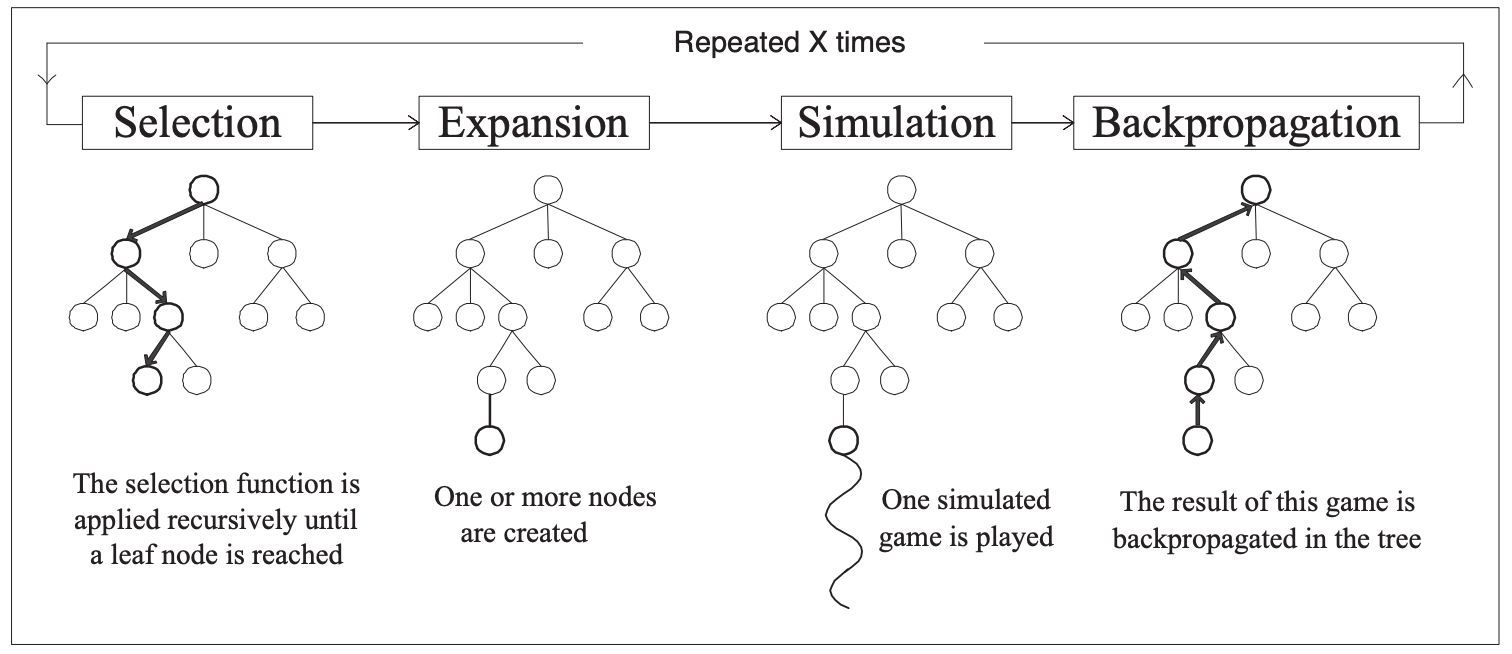
\includegraphics[scale=0.5]{assets/mcts.png}
    \caption[]{The Monte-Carlo Tree Search Framework}
    \label{fig:mcts}
\end{figure}

\subsubsection{Selection}
Thes selection process starts at the root node and repeats until a leaf node in the current tree is reached.
At each level of the tree, a child node is selected based on a selection formula such as UCT or PUCT.
A selection formula usually has two parts, the exploitation part is based on the evaluation function $E$, and the exploration bonus $B$.
For edges of a parent state $(s, a), ~ a \in \mathcal{A}$ , the selection $I(s)$ is based on
\begin{equation}
    \label{eq:mcts_selection}
    I(s) = \operatorname{argmax}_{a \in \mathcal{A}} \left( E(s, a) + B(s, a) \right)
\end{equation}

The prior score could be based on the value of the child, the accumulated reward of the child, or the prior selection probability based on the policy $\pi(a \mid s)$.
The exploration bonus is usually based on the visit count of the child and the parent.
The more visits a child gets, the less the exploration bonus will be.
For example, the selection in the UCT algorithm is based on
\begin{align*}
    I(s)     & = \operatorname{argmax}_{a \in \mathcal{A}} \left( E(s, a) + B(s, a) \right)  \\
    E(s, a)  & = \frac{V(s)}{N(s, a)}  \\
    B(s, a)  & = \sqrt{\frac{2 * \log(n_b)}{n_c}}
\end{align*}
where $v_c$ is the value of the node, $n_b$ and $n_c$ are the visit counts of the parent and child, respectively.
This \citeauthor{ModificationUCTPatterns_Gelly.Wang.ea_2006} used this selection rule in their implementation of MoGo,
the first computer Go program that uses UCT \cite{ModificationUCTPatterns_Gelly.Wang.ea_2006}.

\subsubsection{Expansion}
The selected leaf node is expanded by adding one or more children, each child represents a successor game state reached by playing one legal move.

\subsubsection{Evaluation}
The expanded node is evaluated by playing a game with a rollout policy, using an evaluation function, or using a blend of both approaches.
Many MCTS algorithms use a random policy as the rollout policy and the game result as the evaluation.
Early work on evaluation functions focused on hand-crafted heuristic functions based on experted knowledge.
More recently, evaluation functions are mostly approximated by deep neural networks specifically trained for the problems.
\note{add two examples here}

\note{I'm not sure if using bullets points is appropriate. I also tried using in-line number list (e.g., (1) ..., (2) ..., )}

\subsubsection{Backpropagation}
After the expanded nodes are evaluated, the nodes on the path from the expanded nodes back to the root are updated.
The statistics updated usually include visit count, estimated value and accumulated reward of the nodes.

\subsubsection{MCTS Iteration and Move Selection}
The four steps are repeated until the budget runs out.
After the search, the agent acts by selecting the action associated with the most promising child of the root node.
This could be the most visited child, the child with the greatest value, or the child with the highest lower bound \cite{FreshMaxLcb_RoyJonathan_2019}.

\subsection{AlphaGo}
In \citeyear{MasteringGameGo_Silver.Schrittwieser.ea_2017},
\citeauthor{MasteringGameGo_Silver.Schrittwieser.ea_2017} developed \textbf{AlphaGo},
the first Go program that beats a human Go champion on even terms \cite{MasteringGameGo_Silver.Schrittwieser.ea_2017}.
% AlphaGo learns a policy net that maps states to actions, and a value net that maps states to values.
AlphaGo was trained with a machine learning pipeline with multiple stages.
For the first stage of training, a supervised learning policy (or SL policy) is trained to predict expert moves using a neural network.
This SL policy $p$ is parametrized by weights $\sigma$, denoted $p_{\sigma}$.
The input of the policy network is a representation of the board state, denoted $s$.
Given a state $s$ as the input, this network outputs a probability distribution over all legal moves $a$ through the last softmax layer.
During the training of the network, randomly sampled expert moves are used as training targets.
\note{I'm not sure if I should use past tense. I think I am describing how AlphaGo works as an algorithm (which I think is timeless), not the acutal AlphaGo software that beats Lee.}
The weights $\sigma$ are then updated through gradient ascent to maximize the probability of matching the human expert move:
$$
    \Delta \sigma \propto \frac{\partial \log p_{\sigma}(a \mid s)}{\partial \sigma}
$$
For the second stage of training, the supervised policy $p_{\sigma}$ is used as the starting point for training with reinforcement learning.
This reinforcement learning trained policy (or RL policy) is parametrized by weights $\rho$ so that $p_{\rho} = p_{\sigma}$.
Training data is generated in form of self-play games using $p_{\rho}$ as the rollout policy.
For each game, the game outcome $z_t = \pm r(s_T)$, where $s_T$ is the terminal state, $z_T = +1$ for winning, $z_T = -1$ for losing from the perspective of the current player.
Weights $\rho$ are updated using gradient ascent to maximize the expected outcome using the update formula:
$$
    \Delta \rho \propto \frac{\partial \log p_{\rho}\left(a_{t} \mid s_{t}\right)}{\partial \rho} z_{t}
$$
For the last stage, a value function is trained to evaluate board positions.
This value function is modeled with a neural network with weights $\theta$, denoted $v_{\theta}$.
Given a state $s$, $v_{\theta}(s)$ predicts the outcome of the game if both players act according to the policy $p_{\rho}$.
This neural network is trained with stochastic gradient descent to minimize the mean squared error (MSE) between the predicted value $v_{\theta}(s)$ and the outcome $z$.
$$
    \Delta \theta \propto \frac{\partial v_{\theta}(s)}{\partial \theta}\left(z-v_{\theta}(s)\right)
$$

AlphaGo combines the policy network $p_{\rho}$ and the value network $v_{\theta}$ with MCTS for acting.
AlphaGo uses a MCTS variant similar to that described in \ref{sec:mcts}.
In the search tree, each edge $(s, a)$ stores an action value $Q(s, a)$, a visit count $N(s, a)$, and a prior probability $P(s, a)$.
At each time step, the search starts at the root node and simulates until the budget runs out.
In the select phase of each simulation, an action is selected for each traversed node using the same base formula (\ref{eq:mcts_selection}).
In AlphaGo, the exploitation score of the selection formula is the estimated value of the next state after taking the actions, namely $Q(s, a)$.
The exploration bonus of edge $(s, a)$ is based on the prior probability and decays as its visit count grows.
\begin{equation}
    u(s, a) \propto \frac{P(s, a)}{1 + N(s, a)}
\end{equation}

The action taken at time $t$ maximizes the sum of the exploitation score and the exploration bonus
\begin{equation}
    a_{t}=\underset{a}{\operatorname{argmax}}\left(Q\left(s_{t}, a\right)+u\left(s_{t}, a\right)\right)
\end{equation}

AlphaGo evalutes a leaf node state $s_L$ by blending both the value network estimation $v_\theta(s_L)$ and the game result $z_L$ obtained by the rollout policy $p_\pi$
The mixing parameter $\lambda$ is used to balance these two types of evaluations into the final evaluation $V_(s_L)$
$$
    V\left(s_{L}\right)=(1-\lambda) v_{\theta}\left(s_{L}\right)+\lambda z_{L}
$$

\subsection{AlphaGo Zero}
\textbf{AlphaGo Zero} is a successor of AlphaGo that beat AlphaGo 100-0 \cite{MasteringGameGo_Silver.Schrittwieser.ea_2017}.
The first step in the AlphaGo machine learning pipeline is to learn from human expert moves.
In constrast, AlphaGo Zero learns to play Go \textit{tabula rasa}.
This means it learns solely by reinforcement learning from self-play, starting from random play, without supervision from human data.

Central to AlphaGo Zero is a deep neural network $f_\theta$ with parameters $\theta$.
Given a state $s$ as an input, then network output both move probabilities $\pmb{p}$ and value estimation $v$
$$(\pmb{p}, v) = f_\theta(s)$$.
To generate self-play games $s_1, ..., s_T$, an MCTS is performed at each state $s$ using the latest neural network $f_\theta$.
To select a move for a parent node $p$ in the search tree, a variant of the PUCT algorithm is used
\begin{align*}
    I(s)     & = \operatorname{argmax}_{a \in \mathcal{A}} \left( E(s, a) + B(s, a) \right)  \\
    E(s, a)  & = Q(s, a)  \\
    B(s, a)  & \propto P(s, a) \frac{\sqrt{N(s)}}{1+N(s, a)}
\end{align*}

Self-play games are processed into training targets to update the parameters $\theta$ through gradient descent on the loss function $l$
\begin{equation*}
    l = (z-v)^{2} - \pmb{\pi}^{\mathrm{T}} \log \pmb{p}+c\|\theta\|^{2}
\end{equation*}
where $(z-v)^2$ is the mean squared error regressing on value prediction,
$-\pmb{\pi}^{\mathrm{T}} \log \pmb{p}$ is the cross-entropy loss over move probabilities,
and $c\|\theta\|^2$ is the L2 weight regularization.

\note{I want to say everything else I don't mention here is pretty much like AlphaGo, how do I say that?}

\subsection{AlphaZero}
\textbf{AlphaZero} reduces game specific knowledge of AlphaGo Zero so that the same algorithm could be also applied to Shogi and chess
\cite{MasteringChessShogi_Silver.Hubert.ea_2017}.
One difference between AlphaZero and AlphaGo Zero is that AlphaZero the game result is no
longer either winning or losing ($z \in \{ -1, +1 \}$), but also could be a draw ($z \in \{-1, 0, +1 \}$).
This adaptation takes account of games like chess have a draw condition.
\note{The AlphaGo Zero I described above has little Go-specific information already. I don't know how to put it here.}

\subsection{MuZero} \label{sec:muzero}
In \citeyear{MasteringAtariGo_Schrittwieser.Antonoglou.ea_2020},
\citeauthor{MasteringAtariGo_Schrittwieser.Antonoglou.ea_2020} developed
\textbf{MuZero}, an algorithm that learns to play Atari, Go, chess and Shogi at superhuman level.
Compared to the AlphaGo faimily algorithms,
MuZero has less game specific knowledge and has no access to a perfect model.
MuZero plans with a neural network that learns the game dynamics through experience.
Since MuZero does not make the assumption of having access to a perfect model,
MuZero could be applied to games where either the perfect model is not known or is infeasible to compute with.

MuZero's model has three main functions.
The \textbf{representation function} $h$ encodes a history of observations $o_1, o_2, ..., o_t$ into a hidden state $s_t^0$.
The \textbf{dynamics function} $g$,
given a hidden state $s^k$ and action $a^k$, produces an immediate reward $r^k$ and the next hidden state $s^{k+1}$.
The \textbf{prediction function} $f$,
given a hidden state $s^k$, produces a probability distribution $p^k$ of actions and a value associated to that hidden state $v^k$.
These functions are approximated jointly in a neural network with weights $\theta$
\begin{align}
    x^0_t               & = h_{\theta}(o_1, o_2, ..., o_t) \label{eq:muzero_h}  \\
    (x^{k+1}, r^{k+1})  & = g_{\theta}(x^k, a^k)  \label{eq:muzero_g}  \\
    (v^k, \pmb{p}^k)    & = f_{\theta}(x^k) \label{eq:muzero_f}
\end{align}

MuZero plans with a search method based on the MCTS framework (discussed in \ref{sec:mcts}).
Due to the lack of access to a perfect model, MuZero's MCTS differs from a standard one in numerous ways.
The nodes are no longer perfect representations of the board states.
Instead, each node is associated with a hidden state $s$ as a learned representation of the board state.
The transition is no longer made by the perfect model but the dynamics function $g$.
Moreover, since the dynamics function also predicts a reward, edges created through inferencing with the dynamics function also contribute to the $Q$ value estimation.
% That is, traditionally we have $Q(s, a) = \mathit{E} \left[ V(S_{t + 1}) \mid S_t = s, A_t = a \right]$.

To act in the environment, MuZero plans following the MCTS framework described in section \ref{sec:mcts}.
At each timestep $t$, $s^0_t$ is created using (\ref{eq:muzero_h}).
% To select an action following the MCTS selection template equation , 
A variant of PUCT is used to select an action during the search
\begin{align*}
    I(s)     & = \argmax{a \in \mathcal{A}} \left( E(s, a) + B(s, a) \right)  \\
    E(s, a)  & = Q(s, a)  \\
    B(s, a)  & \propto P(s, a) \frac{\sqrt{N(s)}}{1+N(s, a)}\left[c_{1}+\log \left(\frac{N(s)+c_{2}+1}{c_{2}}\right)\right]
\end{align*}
where $c_1$ and $c_2$ are two constants that adjust the exploration bonus.
The selected edge $(s^k, a^k)$ at depth $k$ is expanded using (\ref{eq:muzero_g}) and evaluated using (\ref{eq:muzero_f}).
At the end of the simulation, the statistics of the nodes along the search path are updated.
Notice since the transitions of the nodes are approximated by the neural network, the search is performed over hypothetical trajectories without using a perfect model.
Finally, the action $a^0$ of the most visited edge $(s^0, a^0)$ of the root node is selected as the action to take in the environment.

Experience generated are stored in a replay buffer and processed to training targets.
The three functions of the model are trained jointly using the loss function
\begin{equation}
    \mathcal{L}_{t}(\theta)=
    \underbrace{\sum_{k=0}^{K} l^{\mathrm{p}}\left(\pi_{t+k}, p_{t}^{k}\right)}_{\circled{1}}
    +
    \underbrace{\sum_{k=0}^{K} l^{\mathrm{v}}\left(z_{t+k}, v_{t}^{k}\right)}_{\circled{2}}
    +
    \underbrace{\sum_{k=1}^{K} l^{\mathrm{r}}\left(u_{t+k}, r_{t}^{k}\right)}_{\circled{3}}
    +
    \underbrace{c\|\theta\|^{2}}_{\circled{4}}
\end{equation}
where $K$ is the number of rollout depth, \circled{1} is the loss of the predicted prior move probabilities and move probabilities imporved by the search, \circled{2} is the loss of the predicted value and experienced n-step return,
\circled{3} is the loss of the predicted reward and the experienced reward, and finally \circled{4} is the L2 regularization.

% In addition to the training samples generated by game play,
\textbf{MuZero Reanalyze} is also used to generate training targets in addition to those generated through game play.
MuZero Reanalyze re-executes MCTS on old games using the latest parameters and generates new training targets with potentially improved policy.
\subsection{Atari Games Playing}
\subsubsection{Atari Learning Environment}
\citeauthor{ArcadeLearningEnvironment_Bellemare.Naddaf.ea_2013a} introduced the \textbf{Arcade Learning Environment (ALE)} \cite{ArcadeLearningEnvironment_Bellemare.Naddaf.ea_2013a}.
ALE provided interfaces of over a hunderd of Atari game environments.
Each ALE environment had specifications on visual representation, action space, and reward signals.
This made ALE environments suitable for machine learning research,
as data were well-represented and evaluation metrics were clearly defined.
Moreover, ALE encouraged researchers to develop generalized algorithms that could learn in multiple environments.

\subsubsection{Deep Q-Networks}
\citeauthor{PlayingAtariDeep_Mnih.Kavukcuoglu.ea_2013} pioneered the study of using deep neural networks to learn in ALE envrionments \cite{PlayingAtariDeep_Mnih.Kavukcuoglu.ea_2013}.
They developed the algorithm \textbf{Deep Q-Networks (DQN)} that learned to play seven of the Atari games and reached human-level performance.
The DQN agent had a neural network that approximates the $Q$ function, parametrized by neural network weights $\theta$, denoted $Q_\theta$.
Experiences were generated through interacting with the environment by taking the action that maximizes the immediate $q$ value
\begin{align*}
    \pi(a_t \mid (o_{t - L - 1}, \dots, o_t)) = \argmax{a}{Q_{\theta}(o_{t - L - 1}, \dots, o_t, a)}
\end{align*}
where $L$ is the length of history, and $o_t$ is the partially observable frame provided by the environment at timestep $t$ (also see \ref{sec:history_stacking}).
Generated experience were stored in an experience replay represented by a FIFO queue.
For each training step, a batch of uniformly sampled experience was drawn from the experience replay, and the loss was computed using
\begin{equation*}
    \mathcal{L}(\theta) \propto \mathbb{E}_\pi\left[r + \gamma \max _{a'} Q_{\theta'}(s', a') - Q_{\theta}(s, a) \right]
\end{equation*}
where $Q_{\theta'}$ were network parameters that updated less frequently than $\theta$.

\subsubsection{Double Q Learning}
\citeauthor{DoubleQlearning_Hasselt_2010} analyzed the overestimation problem of Q values in Q-learning and developed the \textbf{double Q learning}.
Central to double Q-learning was the double Q update that replaced the traditional Q update \cite{DoubleQlearning_Hasselt_2010}.
Double Q learning reduced the overestimation problem by introducing an additional Q estimator and updating two estimator using each other
\begin{align*}
    Q^{A}(s, a) \leftarrow Q^{A}(s, a)+ \alpha \left(r+\gamma Q^{B}\left(s', \argmax{a'}{Q^A(s', a')}\right)-Q^{A}(s, a)\right)  \\
    Q^{B}(s, a) \leftarrow Q^{B}(s, a)+ \alpha \left(r+\gamma Q^{A}\left(s', \argmax{a'}{Q^B(s', a')}\right)-Q^{B}(s, a)\right)
\end{align*}
where $Q^A$ and $Q^B$ were two different Q estimators updated alternatively.
\citeauthor{DeepReinforcementLearning_Hasselt.Guez.ea_2016} followed up by applying the double Q learning in DQN \cite{DeepReinforcementLearning_Hasselt.Guez.ea_2016}.
Similar to the double Q update above, double Q update for neural networks was formulated as
\begin{align*}
    \mathcal{L}(\theta^A)  & \propto \mathbb{E}_\pi \left[ r + \gamma Q_{\theta^B}\left(s', \argmax{a'}{Q_{\theta^A}(s', a')} \right) - Q_{\theta^A}(s, a) \right]  \\
    \mathcal{L}(\theta^B)  & \propto \mathbb{E}_\pi \left[ r + \gamma Q_{\theta^A}\left(s', \argmax{a'}{Q_{\theta^B}(s', a')} \right) - Q_{\theta^B}(s, a) \right]  \\
\end{align*}
where $Q_{\theta^A}$ and $Q_{\theta^B}$ were two sets of parameters of the same neural network architecture.

\subsubsection{Experience Replay}
\citeauthor{PrioritizedExperienceReplay_Schaul.Quan.ea_2016} studied the role of experience reply in DQN and developed the \textbf{prioritized experience replay} \cite{PrioritizedExperienceReplay_Schaul.Quan.ea_2016}.
In the original work of DQN, all samples were drawn from the experience replay uniformly.
In a prioritized experience replay, however, samples were drawn according to a distribution based on their calculated priority
\begin{align*}
    P(i)=\frac{p_{i}^{\alpha}}{\sum_{k} p_{k}^{\alpha}}
\end{align*}
where $P(i)$ was the probability of of $i$-th sample being drawn, $\alpha$ was a constant, and $p_i$ is the priority of the sample.
\citeauthor{PrioritizedExperienceReplay_Schaul.Quan.ea_2016} suggested two approaches to compute priorities of samples.
The first one was \textbf{proportional experience replay}, in which the priority $p$ of sample $i$ was calculated by
\begin{align*}
    p_i = \left|\delta_{i}\right|+\epsilon
\end{align*}
where $\delta_{i}$ was the temporal-difference error of the sample, and $\epsilon$ was a small constant to give all samples a probability to be drawn.
The second one was \textbf{rank-based experience replay}, in which the same temporal difference was calculated, but the final priority was based on the rank of the error,
\begin{align*}
    \text{score($i$)}  & = \left|\delta_{i}\right|+\epsilon  \\
    \text{rank($i$)}   & = \text{index  $i$ of} \operatorname{argsort}(-\text{score($j$) for $j$ in all samples} )  \\
    p_{i}              & = \frac{1}{\operatorname{rank}(i)}
\end{align*}
\citeauthor{DistributedPrioritizedExperience_Horgan.Quan.ea_2018} followed up by implementing a distributed version of the prioritized experience replay \cite{DistributedPrioritizedExperience_Horgan.Quan.ea_2018}.
\citeauthor{RECURRENTEXPERIENCEREPLAY_Kapturowski.Ostrovski.ea_2019} investigated the challenges of using experience replaies for RNN-based agents and developed \textbf{Recurrent Replay Distributed DQN}.

\subsubsection{Network Architectures}
\citeauthor{DuelingNetworkArchitectures_Wang.Schaul.ea_} studied an alternative neural network architecture for ALE learning \cite{DuelingNetworkArchitectures_Wang.Schaul.ea_}.
They developed the \textbf{Dueling Q-network}, that while retaining the inputs and outputs specifications of the Q-network used in DQN, structually represented the learning of the advantage function $A(s, a)$ defined as
\begin{align*}
    A(s, a) = Q(s, a) - V(s)
\end{align*}
The Q-network was parametrized by $\theta$ that could be futher divided into three parts:
$\theta^\text{trunk}$, the shared trunk of the network; $\theta^A$, the advantage head; and $\theta^\text{V}$, the value head.
The network approximated the value function internally going through the shared trunk and the value head, denoted $V_{\theta^{\text{trunk}, V}}$, and the advantage function, denoted $A_{\theta^{\text{trunk}, A}}$.
The values computed by the two heads were combined to form the Q-value as follows
\begin{align*}
    Q_{\theta^{\text{trunk, V, A}}}(s, a)
    = V_{\theta^{\text{trunk, V}}}(s)
    + \left( A_{\theta^{\text{trunk,A}}}(s, a)
    - \frac{1}{| \mathcal{A} | } \sum_{a'}A_{\theta^{\text{trunk},A}}(s, a') \right)
\end{align*}
Similar to DQN, the dueling Q-network was trained through fitting to emperical data generated by interacting with the environment.

\subsection{Scalar Transformation} \label{sec:scalar_transform}
\citeauthor{ObserveLookFurther_Pohlen.Piot.ea_2018} introduced a few enhancements to achieve stable training in Atari games \cite{ObserveLookFurther_Pohlen.Piot.ea_2018}.
We will focus on the \textbf{transformed Bellman Operator} since MuZero and our project used a similar transformation operator.
For different Atari games, reward signals could vary drastically both in density and scale.
This led to high variance in training targets during training of the algorithms, causing algorithms to have difficulty converging.
\citeauthor{PlayingAtariDeep_Mnih.Kavukcuoglu.ea_2013} cliped the reward signal to a range of $[-1, 1]$ to reduce such variance in DQN \cite{PlayingAtariDeep_Mnih.Kavukcuoglu.ea_2013}.
However, this clipping discarded information regarding the scale of rewards and consequently changed the set of optimal policies.
The transformed Bellman Operator was developed to address this problem.
The $Q$ update of the new operator was defined as
\begin{align*}
    % Q^{A}(s, a) \leftarrow Q^{A}(s, a)+ \alpha \left(r+\gamma Q^{B}\left(s', \argmax{a'}{Q^A(s', a')}\right)-Q^{A}(s, a)\right)  \\
    Q(s, a) \leftarrow Q(s, a) + \alpha \phi \left(r +\gamma \max _{a' \in \mathcal{A}} \phi^{-1}\left(Q\left(s', a'\right)\right)\right)
\end{align*}
where $\phi$ is an invertible transformation
\begin{align*}
    \phi(x)       & = \operatorname{sign}(x)\left(\sqrt{|x|+1}-1\right)+\varepsilon x  \\
    \phi^{-1}(x)  & = \operatorname{sign}(x)\left(\left(\frac{\sqrt{1+4 \varepsilon(|x|+1+\varepsilon)}-1}{2 \varepsilon}\right)^{2}-1\right)
\end{align*}
This transformation was also used in MuZero to transform both value targets and reward targets.

\subsubsection{MinAtar}

\subsubsection{Consistency Loss}
\cite{VisualizingMuZeroModels_deVries.Voskuil.ea_2021} \cite{MasteringAtariGames_Ye.Liu.ea_2021} \cite{ObserveLookFurther_Pohlen.Piot.ea_2018}

\cite{MinAtarAtariInspiredTestbed_Young.Tian_2019}
\cite{RainbowCombiningImprovements_Hessel.Modayil.ea_2018}
% \subsubsection{Systems}
% \cite{RayDistributedFramework_Moritz.Nishihara.ea_2018}
% \cite{AcmeResearchFramework_Hoffman.Shahriari.ea_a}
% \cite{AsynchronousMethodsDeep_Mnih.Badia.ea_2016}
% \cite{SEEDRLScalable_Espeholt.Marinier.ea_2020}
% \cite{IMPALAScalableDistributed_Espeholt.Soyer.ea_2018}

\section{Problem Definition}
\note{(5 pages)}

\subsection{Markov Decision Process and Agent-Environment Interface}
\note{this section should be in the introduction, since it defines too many things that we need for later.}

A RL problem is usually represented as a \textbf{Markov Decision Process (MDP)}.
MDP is tuple of four elements where $\mathcal{S}$ is a set of states that forms the \textbf{state space}
$\mathcal{A}$, is a set of actions that forms the \textbf{action space};
$P(s, a, s') = Pr[ S_{t+1} = s' \mid  S_t = s, A_t = a]$ is the \textbf{transition probability function};
$R(s, a, s')$ is the \textbf{reward function}.
To solve a problem formulated as an MDP, we implement the \textbf{Agent-Environment Interface} (Figure \ref{fig:agent_environment_interface}).
The MDP is represented as the \textbf{environment}.
The decision maker that interacts with the environment is called the \textbf{agent}.
At each time step $t$, the agent starts at state $S_t \in \mathcal{S}$, takes an action $A_t \in \mathcal{A}$,
transitions to state $S_{t+1} \in \mathcal{S}$ based on the transition probability function $P(S_{t+1} \mid S_t, A_t)$,
and receives a reward $R(S_t, A_t, S_{t+1})$.
These interactions yield a sequence of actions, states, and rewards $S_{0}, A_{0}, R_{1}, S_{1}, A_{1}, R_{2}, \dots$.
We call this sequence a \textbf{trajectory}.
When a trajectory ends at a terminal state $S_T$ at time $t = T$, this sequence is completed and we called it an \textbf{episode}.

\begin{figure}[ht]
    \centering
    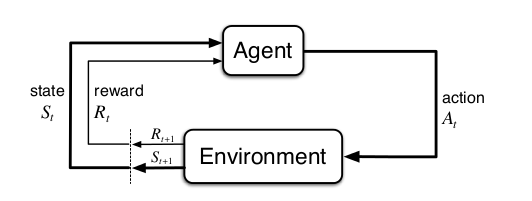
\includegraphics[scale=0.5]{assets/agent_environment_interface.png}
    \caption[]{Agent-Environment Interface}
    \label{fig:agent_environment_interface}
\end{figure}
\note{my notation is messed up but I will fix them later for sure.}

At each state $s$, then agent takes an action based on its \textbf{policy} $\pi(a \mid s)$.
This policy represents the conditional probability of the agent taking an action given a state so that
$\pi(a \mid s) = Pr[ A_{t} = a \mid  S_t = s]$.
One way to specify the goal of the agent is to obtain a policy that maximizes the sum of expected reward from any state $s$
\begin{align}
    \label{eq:maximize_reward_undiscounted}
    \mathit{E}_{\pi}\left[\sum_{k=0}^{T}  R_{t+k+1} \mid S_t = s\right]
\end{align}
where $\mathit{E}_{\pi}$ denotes the expectation of the agent following policy $\pi$.
Another way is to also use a discount factor $\gamma$ so to favor short-term rewards
\begin{align}
    \label{eq:maximize_reward_discounted}
    \mathit{E}_{\pi}\left[\sum_{k=0}^{T} \gamma^{t} R_{t+k+1} \mid S_t = s\right]
\end{align}
Notice that (\ref{eq:maximize_reward_undiscounted}) is a special case of (\ref{eq:maximize_reward_discounted}) where $\gamma = 1$.
\note{Maybe I should use one formula here to unify both.}
% \note{also describes policy $\pi$}
% \note{address this is the most common formulation and how different libraries implement the interface}

% \subsection{Shortcomings of the Agent-Environment Interface for General Game Playing}
% % \note{I'm not sure if I should address these separatly.}
% \subsection{Multi-Agent Games}
% \note{address OpenSpiel's design multiple agents}
% \subsection{Partial Observability}
% \note{address POMDP}
% \subsection{Environment Stochasticity}
% \note{address OpenSpiel's design of random node}
% \subsection{Episodic vs Continuous}
% \note{barely seen in the literature, need more literature review}
% \subsection{Self-Observability}
% % \note{agent needs to be able to observe itself}
% \subsection{Environment Output Structure}
% % The agent-environment interface specifies two return types from the environment, namely the \textbf{observation} and the \textbf{reward}.
% % All environment implementations used in the RL field follow 

\subsection{Our Approach}
\note{(5 pages)}

% The most significant difference of our approach is the separation of data and process.
% In the Agent-Environment Interface, both the agent and the environment are assumed to be stateful, which means they could store and process arbitrary data.

% \subsubsection{Generalized Interaction Interface}
% We propose the \textbf{Generalized Interaction Interface (GII)}.
% We define the \textbf{tape} $E$ as the data storage of the interface, and a \textbf{law} $L$ as a pure function that operates on the tape.
% An instance of such interface could consists of exactly one tape and multiple laws, and we define such an instance a \textbf{universe}.
% A universe \textbf{ticks} by applying the laws on the tape.
% \note{elaborate formally}

% We implement a simplified version of this interface in \textbf{MooZi}.

% % \note{elaborate on the interface}

% \subsubsection{Advantages}
% \note{pure functions are efficient}

\section{Method}
\note{(20 - 25 pages)}
\subsection{Design Philosophy}

% \subsubsection{Use of Generalized Interaction Interface}
% One of the goals of the project is to demostrate the use of Generalized Interaction Interface (GII).
% All modules in the project will be implemented to align with the interface.
% Third-party libraries that include game environments are wrapped with special wrappers that converts the outputs into the GII format.

\subsubsection{Use of Pure Functions}
One of the most notable difference of MooZi implementation is the use of pure functions.
% In GII, \textbf{laws} are pure functions that read from and write to the \textbf{tape}.
% Agents implemented in Agent-Environment Interface usually do not separate the storage of data and the handling of data.
In MooZi, we separate the storage of data and the handling of data whenever possible, especially for the parts with heavy compuations.
For example, we use \textbf{JAX} and \textbf{Haiku} to implement neural network related modules.
These libraries separate the \textbf{specification} and the \textbf{parameters} of a neural network.
The \textbf{specification} of a neural network is a pure function that is internally represented by a fixed computation graph.
The \textbf{parameters} of a neural network includes all variables that could be used with the specification to perform a forward pass.
\note{add one or two more examples of using pure functions, also mention how tape in the MooZi is different from the tape in GII}

% \subsubsection{Being User Friendly}


\subsubsection{Training Efficiency}
One common problem with current open-sourced MuZero projects is their training efficiency.
Even for simple environments, these projects could take hours to train.
\note{
    Data needed; I've seen multiple issues on GitHub complaining about the training speed.
    I once assigned the task of "actually running the project and gather run time data" to Jiuqi but no follow up yet.
}

There are a few major bottlenecks of training efficiency in this type of project.
The first one is system parallelization.
\note{include data from previous presentation to make the point}

The second one is the environment transition speed.
\note{boardgames are fine, Atari games are slow, but in either cases we can't control}
% Board games, especially those are implemented in \textbf{OpenSpiel}, are faster.

The third one is neural network inferences used in training.
\note{MCTS inference batching is slow due to IO overhead, include data here from previous presentation to make the point}

% According to our deGeneralized Interaction Interface
\subsection{Project Structure}

\subsubsection{Overview}
In MooZi, we use \textbf{Ray} library designed by \citeauthor{RayDistributedFramework_Moritz.Nishihara.ea_2018}
for orchestrating distributed processes.
We also adopt the terminology used by Ray \cite{RayDistributedFramework_Moritz.Nishihara.ea_2018}.
In a distributed system with \textbf{centralized control}, a single process is responsible for operating all other processes.
This central process is called the \textbf{driver}.
Other processes are either \textbf{tasks} or \textbf{actors} .
\textbf{Tasks} are stateless functions that takes inputs and return outputs.
\textbf{Actors} are statefull objects that group several methods that take inputs and return outputs.
In RL literature, \textbf{actor} is also a commonly used term for describing the process that holds a copy of the network weights and interacts with an environment \cite{SEEDRLScalable_Espeholt.Marinier.ea_2020}, \cite{IMPALAScalableDistributed_Espeholt.Soyer.ea_2018}.
Even though MooZi does not adopt the concept of a RL actor, we will use the term \textbf{Ray task} and \textbf{Ray actor} to avoid confusion.
In contrast to distributed systems with \textbf{distributed control}, ray tasks and ray actors are reactive and do not have busy loops.
The driver process when a ray task or ray actor is activated and what data should be used as inputs and where the outputs should go.
In other words, the driver process orchestrates the data and control flow of the entire system, and ray tasks and ray actors merely response to instructions, processing inputs and returning outputs on-command.

\begin{figure}[ht]
    \centering
    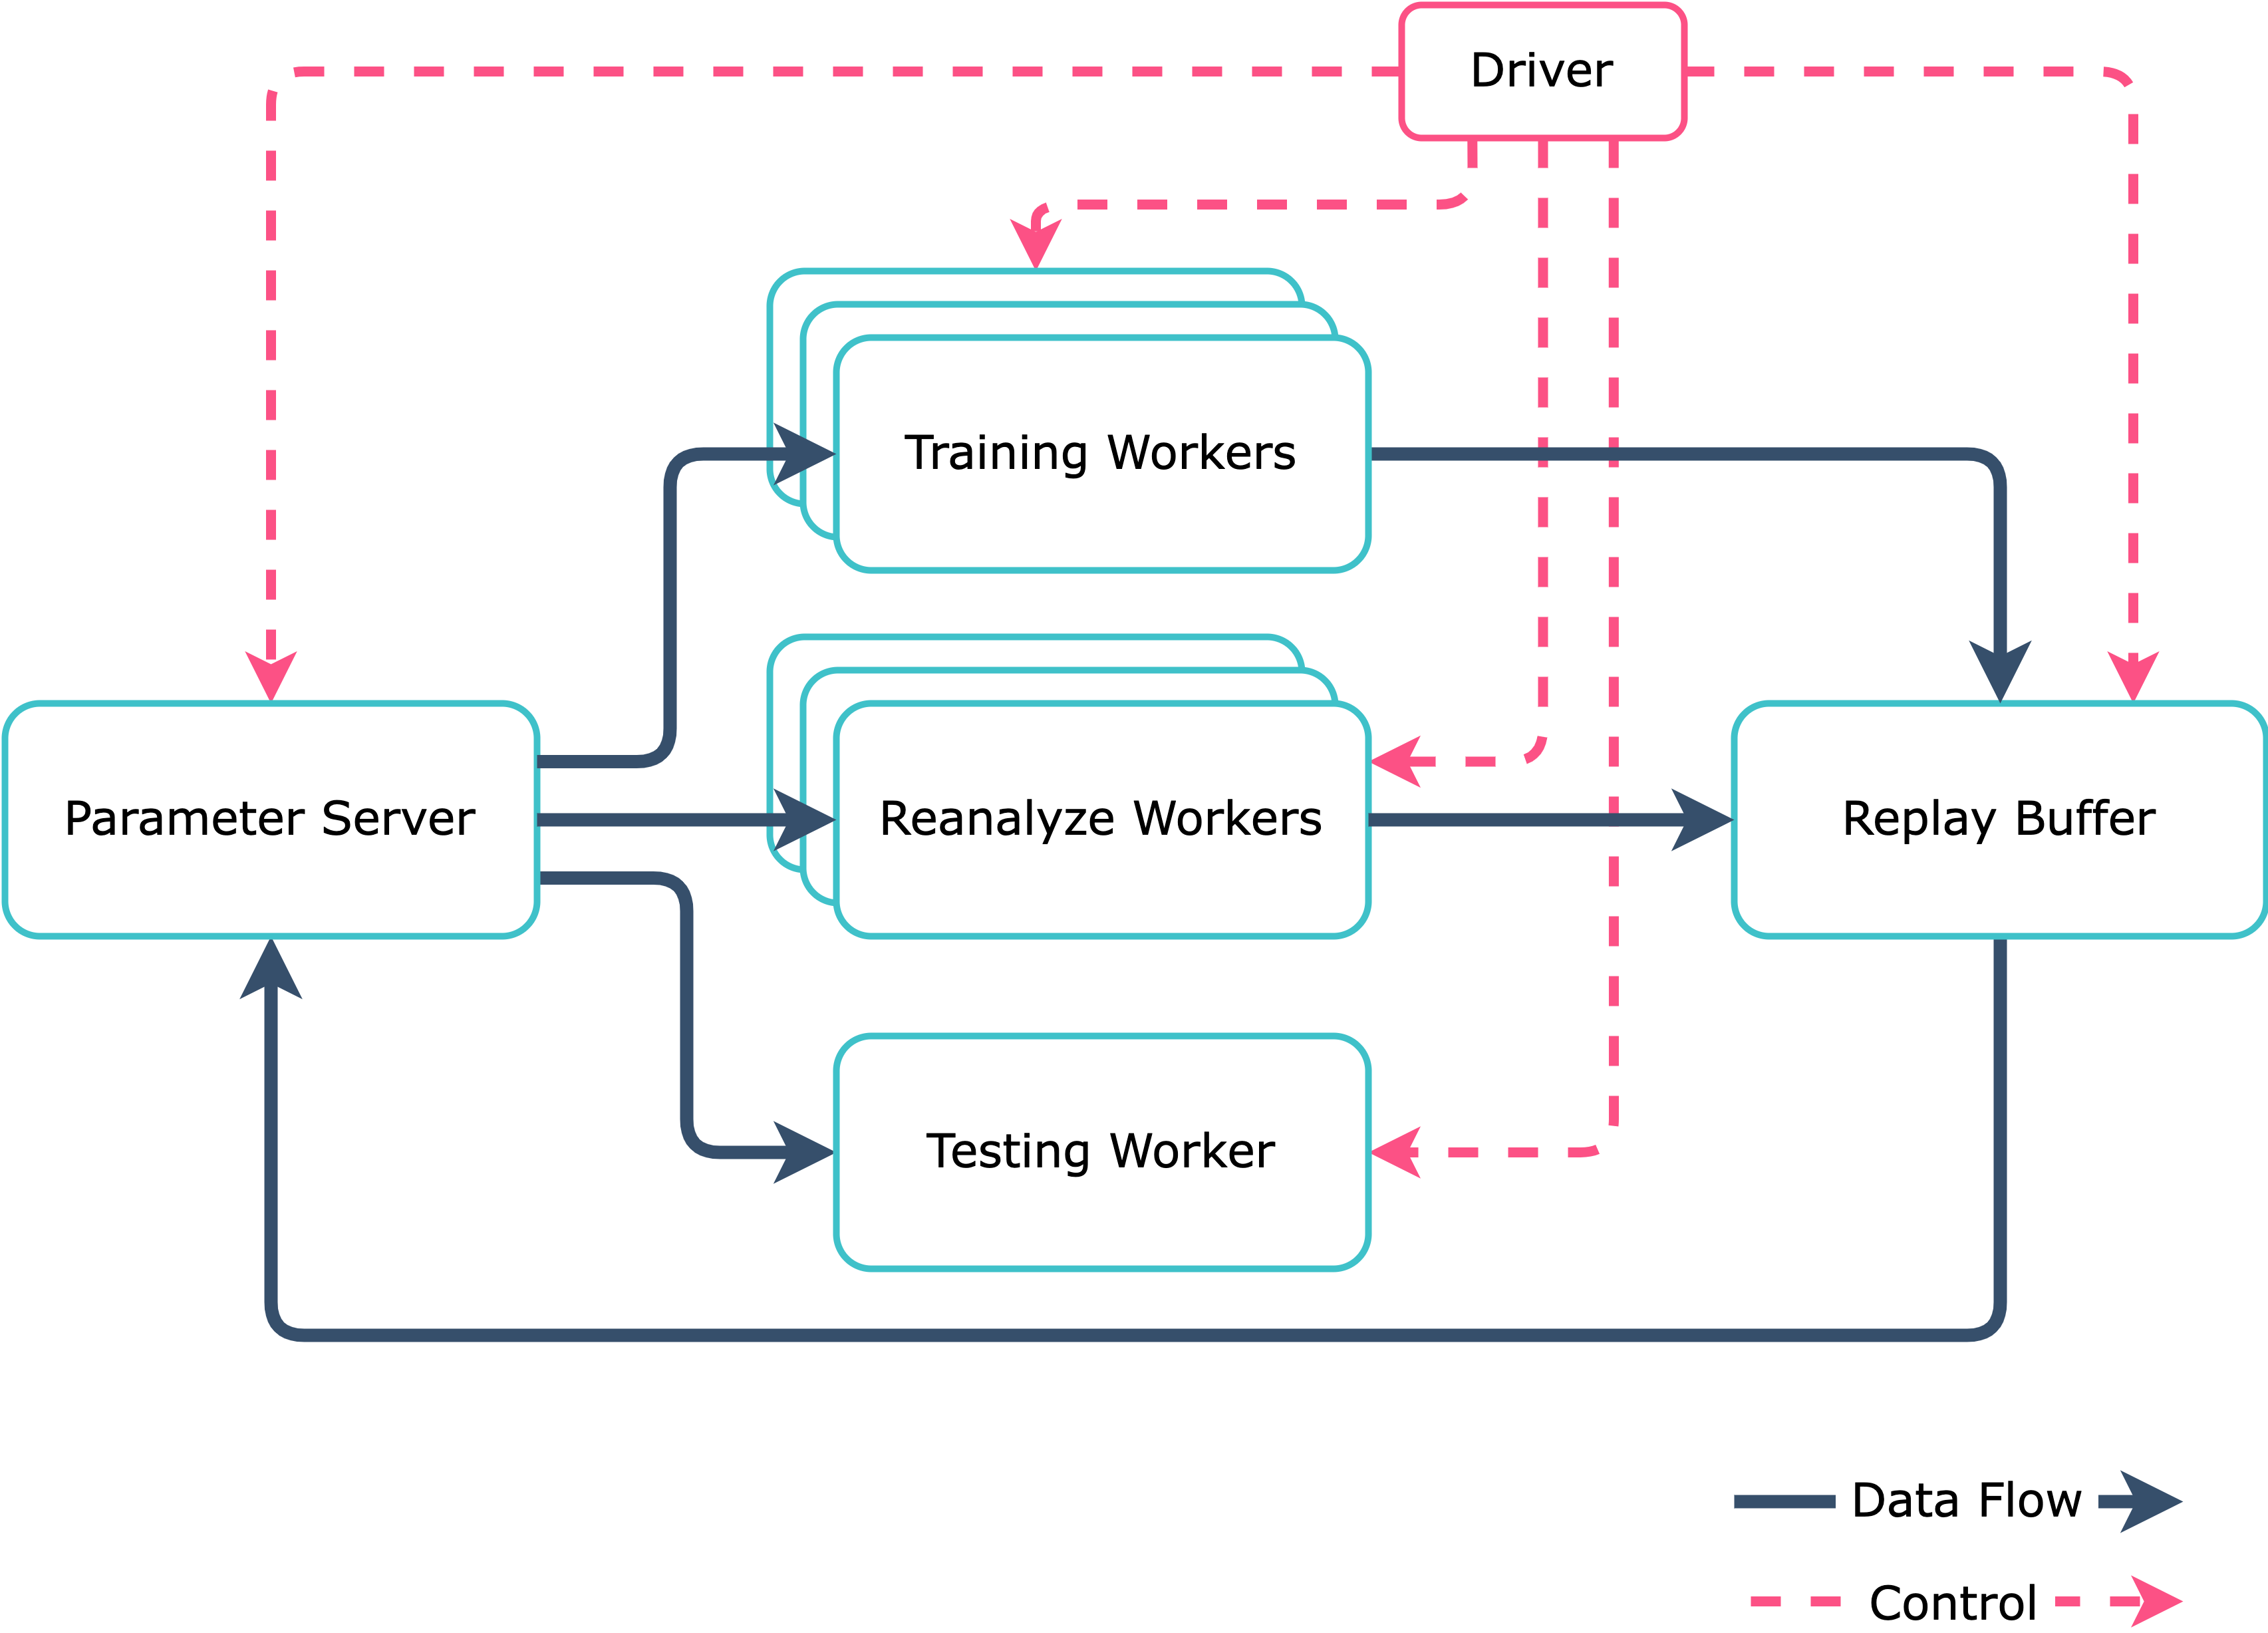
\includegraphics[width=\textwidth]{assets/moozi_architecture.png}
    \caption[]{MooZi Architecture}
    \label{fig:moozi_architecture}
\end{figure}

We illustrate MooZi's architecture design in Figure (\ref{fig:moozi_architecture}).
There are six types of processes.
The \textbf{driver} is the entrance of the program and is responsible for setting up configurations,
spawning other processes as ray actors, and managing data flow among the ray actors.
The \textbf{parameter optimizer} stores the latest copy of the network weights and performs batched updates to the weights.
The \textbf{replay buffer} stores generated trajectories and process the trajectories into training targets.
A \textbf{interaction training rollout worker} is a ray actor that responsible for generating experiences by interacting with the environment.
A \textbf{interaction testing rollout worker} is a ray actor that responsible for evaluating the system (e.g., average episode return) by interacting with the environment.
A \textbf{reanalyze rollout worker} is a ray actor that pulls history trajectories and updates their search statistics using the latest network weights.

\subsubsection{Environment Bridges} \label{sec:env_bridge}
Environment bridges unify environments defined in different libraries into a unified interface.
In the software engineering nomenclature, environment bridges follow the bridge design pattern \cite{BridgePattern__2022}.
More specifically, in our project we implement environment bridges for three types of environments that are commonly used in RL research including OpenAI Gym, OpenSpiel, and MinAtar \cite{OpenAIGym_Brockman.Cheung.ea_2016,OpenSpielFrameworkReinforcement_Lanctot.Lockhart.ea_2020,MinAtarAtariInspiredTestbed_Young.Tian_2019}.
The bridges first wrap these environments into the \textbf{The DeepMind RL Environment API} \cite{DmEnvDeepMind__2022}.
In this format, each environment step outputs a four tuple.
(1) \textbf{step\_type}: an enumerated value indicates the type of the timestep, one of \Verb|first|, the first step in the environment, \Verb|mid|, intermidate steps, and \Verb|last|, the last step in the environment.
(2) \textbf{reward}, a floating point value indicates the reward given by the environment by taking the last given action in the environment.
(3) \textbf{discount}, a floating point value indicates the discount associated with the step.
(4) \textbf{observation}, a data structure represents the new environment observation, could be an N-dimensional array in visual-only observation games, or a nested structure in boardgames where other information such as the next player are represented.
We wrap these environments again to produce a flat dictionary that the rest components in MooZi can use.

The final wrapper environment have the same signature as follows:
\begin{itemize}
    \item Inputs
          \subitem ($b^{\text{last}}_{t}$): A boolean signals the episode end.
          \subitem ($a_t$): An integer indicates the last action taken by the agent.
    \item Outputs
          \subitem ($o_t$):
          An N-dimensional array that represents the observation of the current timestep.
          In the shape of $(H, W, C)$.
          \subitem ($b^{\text{first}}_{t}$): A boolean signals the episode start.
          \subitem ($b^{\text{last}}_{t}$): A boolean signals the episode end.
          %   \subitem  An integer indicates the next player to take a move.
          \subitem $r_t$: A float indicates the reward of taking the given action.
          \subitem $m^{A_a}_t$: A bit mask of legal action indices. Valid
          action indices of $1$ and invalid actions have indices of $0$.
          $ | \mathcal{A_e} | + 1 = | \mathcal{A} | $ (see \ref{sec:a_aug}).
\end{itemize}

All environments are generalized as continuous tasks.
This is done by passing an addition input $b^\text{last}_t$ to the environment stepping argument.
For an episodic task, the environment is reset internally when $b^{\text{last}}_t$ is \Verb|True|.
The policy still executes for the last environment step, but the resulting action is not used by the environment.
For a continuous task, the environment always step with the lastest action and the $b^{\text{last}}_t$ input is ignored.
See \ref{code:env_interface} for pseudo-code of generalizing both types of environments to achieve a unified main loop interface.

Moreover, we also implemented a mock enviornment using the same interface \cite{MockObject__2021}.
A mock environment is initialized with a trajectory sample $\mathcal{T}$, and simulates the environment by outputing step samples one at a time.
An agent could interact with this mock environment as if it is a real environment.
However, the actions taken by the agent would not affect state transitions since they are predetermined by the given trajectory from initialization.
This mock environment is used for reanalyze rollout workers described in \ref{sec:reanalyze_rw}.

\includecode{env_interface}{Environment Adapter Interface}

\subsubsection{Vectorized Environment} \label{sec:vec_env}
We also implement an environment supervisor that stacks multiple individual environments and forms a single vectorized environment.
The resulting vectorized environment takes inputs and produces outputs similar to an individual environment but with an additional batch dimension.
For example, an individual environment produces a single frame of shape $(H, W, C)$ while the vectorized environment produces a batched frame of shape $(B, H, W, C)$.
Previous scalar outputs such as reward are also stacked into vectors with size of $B$.
Since environment adapters generalizes episodic tasks as continuous tasks, we do not need special handling for the first and the last timesteps in the vectorized environment and its main loop looks exactly like that in \ref{code:env_interface}.
Using vectorized environments increases the communication bandwidth between the environment and agent and facilitates designing an vectorized agent that processes a batched of observations and returns a batch of actions at a time.

The mocked environment described in \ref{sec:env_bridge} was less trivial to vectorize.
Each mocked environment has to be initialized with a trajectory sample.
To vectorize the mocked environments of size $B$, at least $B$ trajectories have to be mocked and tracked at the same time.
These $B$ trajectories usually have different length and therefore terminate at different timesteps.
Once one of the mocked trajectory reaches its termination, another trajectory has to fill the slot.
We created a trajectory buffer to address this problem in vectorized mocked environment.
When a new trajectory is needed by one of the mocked environment, the buffer supplies a new trajectory to that mocked environment.
With the trajectory buffer, the vectorized mocked environment could process batched interactions like a regular vectorized environment until the trajectory buffer runs out of trajectory supply.

\subsubsection{Action Space Augmentation} \label{sec:a_aug}
We augmented the action space by adding a dummy action indexed at 0.
This dummy action has two major purposes.
Firstly, this dummy action is to used construct history observations when the horizon is beyond the current timestep.
For example, if the history horizon is 3, we need the last three frames and actions to construct the input observation to the policy.
However, the current timestep could be 0, which means the agent hasn't taken an action yet.
We used zeroed frames with the same shape as history frames, and the augmented dummy action as history actions.
Formally, we define
\begin{align*}
    a_{i}  & = 0 ~~~~ \forall i < 0  \\
    a_{T}  & = 0  \\
\end{align*}

Secondly, since MooZi's planner does not have access to a perfect model, it does not know when a terminal state is reached.
Node expansions do not stop at terminal states and the tree search could simulate multiple steps beyond legal game states.
Search performed in these invalid subtrees not only wastes previous search budget, but also back-propagates value and reward estimates that are not learned from generated experience.
We addressed this issue by letting the model to learn a policy that takes the dummy action beyond terminal states.
The learned dummy action acts as a switch that, once taken, treats all nodes in its subtree as absorting states and edges that have zero values and rewards respectively.

\subsubsection{MooZi Agent}
% \textbf{MooZi Agent} is not a standalone components, but

The MCTS in MooZi Planner was similar to that described in \ref{sec:mcts} and \ref{sec:muzero}.
We used the open-source implementation of MCTS, \textbf{MCTX}, by \citeauthor{POLICYIMPROVEMENTPLANNING_Danihelka.Guez.ea_2022} \cite{POLICYIMPROVEMENTPLANNING_Danihelka.Guez.ea_2022}.
This library was implemented in JAX and supported \note{supports?} customized initial inference and recurrent inference.
We built a simple adapter that connected our neural network interface with MCTX.

\subsubsection{History Stacking} \label{sec:history_stacking}
In fully observable environments, the state $s_t$ at timestep $t$ observed by the agent entails sufficient information about future state distribution.
However, for partially observable environments, this assumption does not hold.
The optimal policy might not be representable by a policy $\pi(a \mid o_t)$ that only takes into account the most recent partial observation $o_t$.
Atari games are usually partially observable environments.
In \textbf{Deep Q Networks (DQN)}, \citeauthor{PlayingAtariDeep_Mnih.Kavukcuoglu.ea_2013} alleviated this problem by augmenting the inputs of the policy network from a single frame observation to a stacked history of four frames so that the policy network had a signature of $\pi(a \mid o_{t-3}, o_{t-2}, o_{t-1}, o_t)$.
AlphaZero and MuZero not only stacked a history of environment frames, but also a history of past actions.
We also adopted this practice in MooZi, and we use the last $L$ environment frames and taken actions so that the signature of the learned model through the policy head is $\pi(a \mid o_{t - L - 1}, \dots, o_t, a_{t - L - 2}, \dots, a_{t-1})$.
$N$ is an adjustable configuration of the MooZi system and in fully observable environments we could set this to $1$.

The exact process of creating the model input by stacking history frames and actions is as follows:
\begin{enumerate}
    \item prepare saved $L$ environment frames of shape $(L, H, W, C_e)$
    \item stack the $L$ dimension with the environment channels dimension $C$, now shape of $(H, W, N * C_e)$
    \item prepare saved $L$ past actions of shape $(L)$, represented as action indices
    \item one-hot encode the actions, now shape of $(L, A)$
    \item stack the $L$ dimension with the action dimension $A$, now shape of $(L * A)$
    \item divide the action planes by the number of action, shape remains the same
    \item tile action planes $(L * A)$ along the $H$ and $W$ dimensions, now shape of $(H, W, N * A)$
    \item stack the environments planes and actions planes, now shape of $(H, W, L * (C_e + A))$
    \item the history is now represented as an image with height of $H$, width of $W$, and $L * (C_e + A)$ channels
\end{enumerate}
To process batched inputs from vectorized environments descirbed in \ref{sec:vec_env}, all operations aboved are performed with an additional batch dimension $B$, yielding the final output with the shape $(B, H, W, L * (C_e + A))$.
We denote the channels of the final stacked history as $C_h$ so that $C_h = N * (C_e + A)$, where the subscript $h$ means the channel dimension for the representation function $h$.

\subsubsection{MooZi Neural Network}
\note{neural network specifical should go into experiment section}
We used JAX, and Haiku to build the neural network \cite{HaikuSonnetJAX_Hennigan.Cai.ea_2020, CompilingMachineLearning_Frostig.Johnson.ea_2018, JAXAutogradXLA_JamesBradbury.RoyFrostig.ea_2022}.
We consulted other open-source projects that use neural networks to play games \cite{MuZeroGeneral_Duvaud.AureleHainaut_2022, MasteringAtariGames_Ye.Liu.ea_2021,AcceleratingSelfPlayLearning_Wu_2020,AcceleratingSelfPlayLearning_Wu_2020}.
We implemented the neural-network model with two different architectures in our project, one is multilayer-perceptron-based and the other one is residual-blocks-based \cite{DeepResidualLearning_He.Zhang.ea_2016}.
We primarily used residual-blocks-based model for experiments so we will describe the architecture in full details here.

Similar to MuZero described in section \ref{sec:muzero}, the model had the representation function, the dynamics function, and the dynamics function.
Additionally, we also trained the MooZi model with a self-consistency loss similar to that described by \citeauthor{MasteringAtariGames_Ye.Liu.ea_2021} and \citeauthor{VisualizingMuZeroModels_deVries.Voskuil.ea_2021} \cite{MasteringAtariGames_Ye.Liu.ea_2021,VisualizingMuZeroModels_deVries.Voskuil.ea_2021}.
We used an additional function, named as the \textbf{projection function} for this purpose.
The learned model was used for two purposes during tree searchs.
The first one was to construct the root nodes using the representation function and the prediction function.
We call this process the \textbf{initial inference}.
The second one was to create edges and child nodes for a given node and action using the dynamics function and the prediction function.
We call this process the \textbf{recurrent inference}.
\note{This terminology is aligned with MuZero's pseudo-code and MCTX's real code}

We implemented residual blocks using the same specification as \citeauthor{DeepResidualLearning_He.Zhang.ea_2016} \cite{DeepResidualLearning_He.Zhang.ea_2016}.
One residual block was defined as follows:
\begin{itemize}
    \item input $x$
    \item save a copy of $x$ to $x'$
    \item apply a 2-D padded convolution on $x$, with kernel size 3 by 3, same channels
    \item apply batch normalization on $x$
    \item apply relu activation on $x$
    \item apply a 2-D padded convolution on $x$, with kernel size 3 by 3, same channels
    \item apply batch normalization on $x$
    \item add $x'$ to $x$
    \item apply relu activation on $x$
\end{itemize}

The representation function $h$ is parametrized as follows:
\begin{itemize}
    \item input $x$ of shape $(H, W, C_h)$
    \item apply a 2-D padded convolution on $x$, with kernel size 3 by 3, 32 channels
    \item apply batch normalization on $x$
    \item apply relu activation on $x$
    \item apply 6 residual blocks with 32 channels on $x$
    \item apply a 2-D padded convolution on $x$, with kernel size 3 by 3, 32 channels
    \item apply batch normalization on $x$
    \item apply relu activation on $x$
    \item output the hidden state head $x_s$ % of shape $(H, W, 32)$
\end{itemize}

The prediction function $f$ is parametrized as follows:
\begin{itemize}
    \item input $x$ % of shape $(H, W, 32)$
    \item apply a 2-D padded convolution on $x$, with kernel size 3 by 3, 32 channels
    \item apply batch normalization on $x$
    \item apply relu activation on $x$
    \item apply 1 residual block with 32 channels on $x$
    \item flatten $x$
    \item apply 1 dense layer with output size of 128 to obtain the value head $x_v$
    \item apply batch normalization on $x_v$
    \item apply relu activation on $x_v$
    \item apply 1 dense layer with output size of $Z$ on $x_v$
    \item apply 1 dense layer with output size of 128 to obtain the policy head $x_p$
    \item apply batch normalization on $x_p$
    \item apply relu activation on $x_p$
    \item apply 1 dense layer with output size of $A^a$ on $x_p$
    \item output the value head $x_v$ and the policy head $x_p$
\end{itemize}

The dynamics function $g$ is parametrized as follows:
\begin{itemize}
    \item input $x$ of shape $(H, W, 32)$, $a$ as an integer
    \item encode $a$ as action planes of shape $(H, W, A)$ (described in \ref{sec:history_stacking})
    \item append $a$ to $x$

    \item apply a 2-D padded convolution on $x$, with kernel size 3 by 3, 32 channels
    \item apply batch normalization on $x$
    \item apply relu activation on $x$

    \item apply 1 residual block with 32 channels on $x$

    \item apply 1 residual block with 32 channels on $x$ to obtain the hidden state head $x_s$
    \item apply a 2-D padded convolution on $x_s$, with kernel size 3 by 3, 32 channels
    \item apply batch normalization on $x_s$
    \item apply relu activation on $x_s$

    \item apply 1 dense layer with output size of 128 on $x$ to obtain the reward head $x_r$
    \item apply batch normalization on $x_r$
    \item apply relu activation on $x_r$
    \item apply 1 dense layer with output size of $Z$ on $x_r$

    \item output the hidden state head $x_s$ and the reward head $x_r$
\end{itemize}
For convinience, we made the output specification the same for both the initial inference and the recurrent inference.
They both produced a tuple of $(x, v, r, p)$, $x$ was the hidden state, $v$ was the value prediction, $r$ was the reward prediction, and $p$ was the policy prediction.
% For acting in an environment, the outputs $v$ and $r$ were 

For the initial inference,
\begin{itemize}
    \item input features $\psi_t = (o_{t - L + 1}, \dots, o_t, a_{t - L}, \dots, a_{t -1})$
    \item obtain $\mathbf{x}_t^0 = h(\psi_t)$
    \item obtain $v^0_t, \mathbf{p}^0_t = f(\mathbf{x}_t^0)$
    \item set $r_t^0 = 0$
    \item return $(\mathbf{x}^0_t, v_t^0, r_t^0, \mathbf{p}^0_t)$
\end{itemize}

For the recurrent inference,
\begin{itemize}
    \item input features $\mathbf{x}_t^i, a_t^i$
    \item obtain $\mathbf{x}_t^{i+1}, r_t^{i+1} = g(s_t^i, a_t^i)$
    \item obtain $v^{i+1}_t, \mathbf{p}^{i+1}_t = f(\mathbf{x}_t^{i+1})$
    \item return $(\mathbf{x}^{i+1}_t, v_t^{i+1}, r_t^{i+1}, \mathbf{p}^{i+1}_t)$
\end{itemize}

Moreover, we applied the invertible transformation \( \phi \) described in section \ref{sec:scalar_transform} to both the scalar reward targets and scalar value targets to create categorical representations with the same support size.
The support we used for the transformation were integers from the interval \( [-5, 5] \), with a total size of 11.
Scalars were first transformed using \( \phi \), then converted to a linear combination of the nearest two integers in the support.
For example, for scalar \(\phi(x) = 1.3\), the nearest two integers in the support are $1$ and $2$, and the linear combination is \( \phi(x) = 1 * 0.7 + 2 * 0.3 \), which means the target of this scalar is $0.7$ for the category $1$, and $0.3$ for the category $2$. 
For training, the value head and the reward head first produced estimations as logits of size $Z$.
These logits were aligned with the scalar targets to produce categorization loss as described in the \ref{sec:loss}.
For acting, the neural network additionally applied the softmax function to the logits to generated a distribution over the support.
The linear combination of the distribution and their corresponding integer values were computed and fed through the inverse of the transformation, namely \( \phi^{-1}\), to produce scalar values.
This means from the perspective of the planner, the scalar estimations made by the model were in same shape and scale as those produced by the environment.

\note{reference an example in the experiments section}


\subsubsection{Training Targets Generation} \label{sec:targets}
% The agent interacted with the environment by taking actions.
At each timestep $t$, the environment provides a tuple of data as described in seciton (\ref{sec:env_bridge}).
The agent interacts with the environment by performing a tree search and taking action $a_t$.
The search statistics of the tree search were also saved, including the updated value estimate of the root action $\hat{v}_t$,
    and the updated action probability distribution $\hat{p}_t$.
These completes one step sample $\mathcal{T}_t$ for timestep $t$, which is a tuple of $(o_t, a_t, b^{\text{first}}_{t}, b^{\text{last}}_{t}, r_t, m^{A_a}_t, \hat{v}_t, \hat{p}_t)$.
Once an episode concludes ($b^{\text{last}}_{T} = 1)$, all recorded step samples are gathered and stacked together.
This yields a final trajectory sample $\mathcal{T}$ that has a similar shape to a step sample but with an extra batch dimension with the size of $T$.
For example, $o_t$ is stacked from shape $(H, W, C_e)$ to shape $(T, H, W, C_e)$.
The interaction training rollout workers described in \ref{sec:train_rw} generate trajectories this way.
The reanalyze rollout workers generate trajectories with the same signature, but through statistics update described in using a vectorized mocked environment (see \ref{sec:reanalyze_rw} and \ref{sec:vec_env}).

Each trajectory sample with $T$ step samples were processed into $T$ training targets.
For each training target at timestep $i$, we create a training target as follows:
\begin{itemize}
    \item Observations $o_{i - H - 1}, \dots, o_{i + 1}$ where $H$ is the history stacking size.
          The first $H$ observations were used to create policy inputs as described in \ref{sec:history_stacking},
          and the pair of observation $o_{i}, o_{i+i}$ were used to compute self-consistency loss described in \ref{sec:loss}.

    \item Actions $a_{i - H - 2}, \dots, a_{i + K - 1}$.
          Similarly, The first $H$ actions were used for policy input and the pair of actions at $(a_{i - 1}, a_{i})$ were used for self-consistency loss.
          The actions $a_{i}, \dots, a_{i + K - 1}$ were used to unroll the model during the training for $K$ steps.

    \item Rewards $r_{i + 1}, \dots, r_{i + K}$ as targets of the reward head of the dynamics function.
    
    \item Action probabilities $\hat{p}_{i}, \dots, \hat{p}_{i + K}$ from the statistics of $K + 1$ search trees.
    
    \item Root values $\hat{v}_i, \dots, \hat{v}_{i + K}$, similarly, from the statistics of $K + 1$ search trees.

    \item N-step return $G^N_{i}, \dots, G^N_{i + K}$.
          Each N-step return was computed based on the formula
          \begin{align*}
              G^N_{t} = \sum_{i = 0}^{i = N - 1}{\gamma^i r_{t+i+1}} + \gamma^N\hat{v}_{t + N}
          \end{align*}
          
    \item Importance sampling ratio $\rho = 1$. Placeholder value for future override based on replay buffer sampling weights (see \ref{sec:replay}).
\end{itemize}

\subsubsection{The Loss Function} \label{sec:loss}
The loss function was defined similar to \ref{sec:muzero}, but with additional self-consistency loss, terminal action loss, $L_2$ regularization loss, and 
\begin{equation}
    \mathcal{L}_{t}(\theta)=
    \underbrace{\sum_{k=0}^{K} l^{\mathrm{p}}\left(\pi_{t+k}, p_{t}^{k}\right)}_{\circled{1}}
    +
    \underbrace{\sum_{k=0}^{K} l^{\mathrm{v}}\left(z_{t+k}, v_{t}^{k}\right)}_{\circled{2}}
    +
    \underbrace{\sum_{k=1}^{K} l^{\mathrm{r}}\left(u_{t+k}, r_{t}^{k}\right)}_{\circled{3}}
    +
    \underbrace{c\|\theta\|^{2}}_{\circled{4}}
\end{equation}


\subsubsection{Rollout Workers}
\textbf{Rollout workers} are ray actors that store copies of environments or history trajectories and generated data by evaluating policies and interacting with the environments or history trajectories.
A rollout worker does not inherently serve a specific purpose in the system and its behavior is mostly determined by the universe factory passed to it.
There are three main types of rollout workers used in MooZi.

\subsubsection{Interaction Training Rollout Worker} \label{sec:train_rw}
The main goal of \textbf{interaction training rollout workers} were to generated trajectories by interacting with environments.
For each worker, a vectorized enviornment was created as described in \ref{sec:vec_env}, a history stacker was created as described in \ref{sec:history_stacking}, and a planner was created using MCTS configurations as described in \ref{sec:planner}:
Step samples and trajectory samples were collected as the vectorized enviornment stepping, and finally collected trajectory samples were returned as the final output of one run of the worker.
See \ref{code:interaction_training_rollout_worker} for the pseudo-code of this process.

\includecode{interaction_training_rollout_worker}{Interaction Training Rollout Worker}

\textbf{Interaction Testing rollout worker},

\subsubsection{Reanalyze Rollout Worker} \label{sec:reanalyze_rw}

\subsubsection{Replay Buffer} \label{sec:replay}

Since most training targets were expected to be sampled more than once, we precomputed the training targets for all received trajectory samples in the replay buffer. 
Training targets were computed with minimum information neccessary to be used in the loss function (see \ref{sec:targets}) so that the precomputation took least memory possible.

The replay buffer:
\begin{itemize}
    \item stores trajectories generated by the rollout workers
    \item processes the trajectories into training targets
    \item stores processed training targets
    \item computes and updates priorities of training targets
    \item responsible for sampling and fetching batches of training targets
\end{itemize}

\subsubsection{Parameter Optimizer}
The parameter optimizer:
\begin{itemize}
    \item stores a copy of the neural network specification
    \item stores the latest copy of neural network parameters
    \item stores the loss function
    \item stores the training state
    \item computes forward and backward passes and updates the parameters
\end{itemize}

\subsubsection{Distributed Training}
\subsubsection{Logging and Visualization}


\section{Experiments}
\note{(20 pages)}

\section{Conclusion}
\note{(3 pages)}
\subsection{Future Work}
\note{(1 page)}

\printbibliography

\end{document}

% \subsection*{Artificial Intelligence}

% % Artificial Intelligence (AI) is a branch of computer science that emphasizes the use of computer algorithms to solve problems likes humans.
% To define the goals and methods of Artificial Intelligence (AI), we first need to define what is \textit{intelligence}.
% Though there is no consensus on the exact definition of intelligence, here we adopt the definition by John McCarthy:
% \begin{quote}
%     Intelligence is the computational part of the ability to achieve goals in the world.
% \end{quote}
% The goal of AI is to develop computer algorithms that can solve problems and achieve goals in complex environments.
% A diverse range of methods are designed as AI algorithms since the term has been coined.
% \note{A simple list of AI algorithms, such as A*, symbolic}


% \subsection*{Game Artificial Intelligence}
% Perfect vs in-Perfect information
% \subsection*{Planning}
% lookahead search: A*, DFS, BFS

% \subsection*{Distributed System for AI}
% IMPALA, SEED
